% carried from the v2 tree (results.tex); the depth/quadrature clause was corrected in v3 to match Sec. 8.
\begin{figure*}[tp]\centering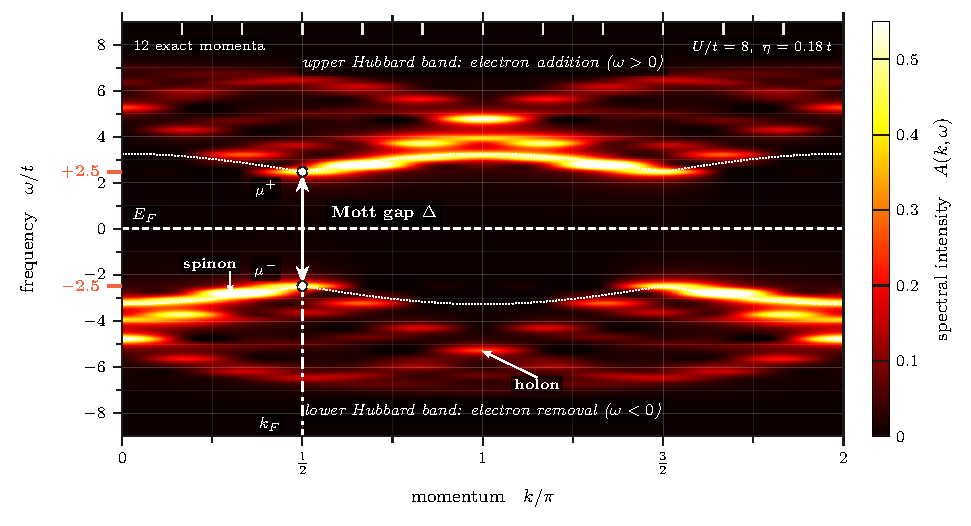
\includegraphics[width=\linewidth]{figs/fig_akw_native.pdf}
\caption{\textbf{Momentum-resolved spectral function: the dynamical target.} The
single-particle spectral function $A(k,\omega)$ of the half-filled Hubbard chain ($U/t=8$, $L=12$,
Lorentzian broadening $\eta=0.18\,t$), computed from the resolvent $\langle\phi|(z-\hat H)^{-1}|\phi\rangle$ by a
Haydock continued fraction~\cite{haydock1972} of depth $n_\ell=150$ over the full $(N{\pm}1)$ sectors---a
finite-depth continued fraction, that is a $150$-node Gauss quadrature of the spectral
measure~\cite{golub2010} and not the Lehmann sum; versions~1--2 called it exact and
Sec.~\ref{sec:physics} withdraws that word---the frequency- and momentum-resolved
observable that sample-based diagonalization targets but its energy-only output cannot itself deliver.
The two dispersing Hubbard bands---electron removal (lower, $\omega<0$; photoemission) and electron
addition (upper, $\omega>0$; inverse photoemission)---are separated by the correlation-driven
\emph{Mott gap} $\Delta=\mu^{+}-\mu^{-}=4.97\,t$ between the highest occupied state ($\mu^{-}$, lower
edge) and the lowest unoccupied state ($\mu^{+}$, upper edge), obtained from the exact $(N{\pm}1)$
ground-state energies (ticks at $\pm2.484\,t$); the broadened spectral peaks of the plotted $A(k_F,\omega)$
sit slightly wider, at $\pm2.49\,t$ (a $4.99\,t$ splitting), the $\sim\!0.02\,t$ excess being the
$\eta=0.18\,t$ Lorentzian broadening; the thermodynamic Lieb--Wu value~\cite{liebwu1968} is $4.68\,t$, the
$L=12$ excess being finite-size. The gap is \emph{direct} at the
Fermi momentum $k_F=\pi/2$. Particle--hole symmetry places the Fermi level at mid-gap ($\omega=0$),
verified to double-precision round-off, and each momentum obeys the analytic spectral sum rule
$\int A(k,\omega)\,d\omega=1$ (the plotted broadened grid recovers it to $\sim\!2\%$ within the $\pm9t$ window).
The lower Hubbard band is not a single quasiparticle branch but \emph{spin--charge separated}:
a narrow spinon branch (bandwidth $\pi J/2=0.79\,t$~\cite{descloizeaux1962}, $J=4t^2/U$; dashed,
validated against the exact peak dispersion to ${<}0.1\,t$) rides a broad holon (charge, ${\sim}4t$)
band---the hallmark fractionalization of the 1D Mott insulator~\cite{liebwu1968}. At $L=12$ that
structure is three to seven poles per momentum (Table~\ref{tab:poles}); the words appropriate to the
thermodynamic limit are not used for it.
The momentum axis is a periodic cubic-spline interpolation of the $12$ physical momenta (ticks, top).
Faithfully \emph{sampling} this full momentum-resolved observable---as opposed to the ground-state
energy---requires a large fraction of the $(N{+}1)$ sector (Fig.~\ref{fig:scaling}), the cost
quantified in Sec.~\ref{sec:prices}.}\label{fig:lattice}\end{figure*}
